\begin{multimuons-1}[enhanced, tikz={rotate=0}]{CDF publishes multi-muons!}
  \begin{multicols}{2}
    We report a study of multi-muon events produced at the
    Fermilab Tevatron collider and recorded by the CDF~II detector. In a data 
    set acquired with a dedicated dimuon trigger and corresponding to an 
    integrated luminosity of 2100 pb$^{-1}$, we isolate a significant sample of 
    events in which at least one of the muon candidates is produced 
    outside of the beam pipe of radius 1.5 cm. The production cross section
    and kinematics of events in which both muon candidates are produced inside
    the beam pipe are successfully modeled by known QCD processes which
    include heavy flavor production. In contrast, we are presently unable to 
    fully account for the number and properties of the remaining events, in which
    at least one muon candidate is produced outside of the beam pipe, in terms
    of the same understanding of the CDF~II detector, trigger, and event 
    reconstruction. Several topological and kinematic properties of these 
    events are presented in this paper. These events offer a plausible 
    resolution to long-standing inconsistencies related to $b\bar{b}$
    production and decay.
    \begin{comment}
    % ========================
    \begin{figure}
      \begin{center}
        \vspace{-0.2in}
        \leavevmode
        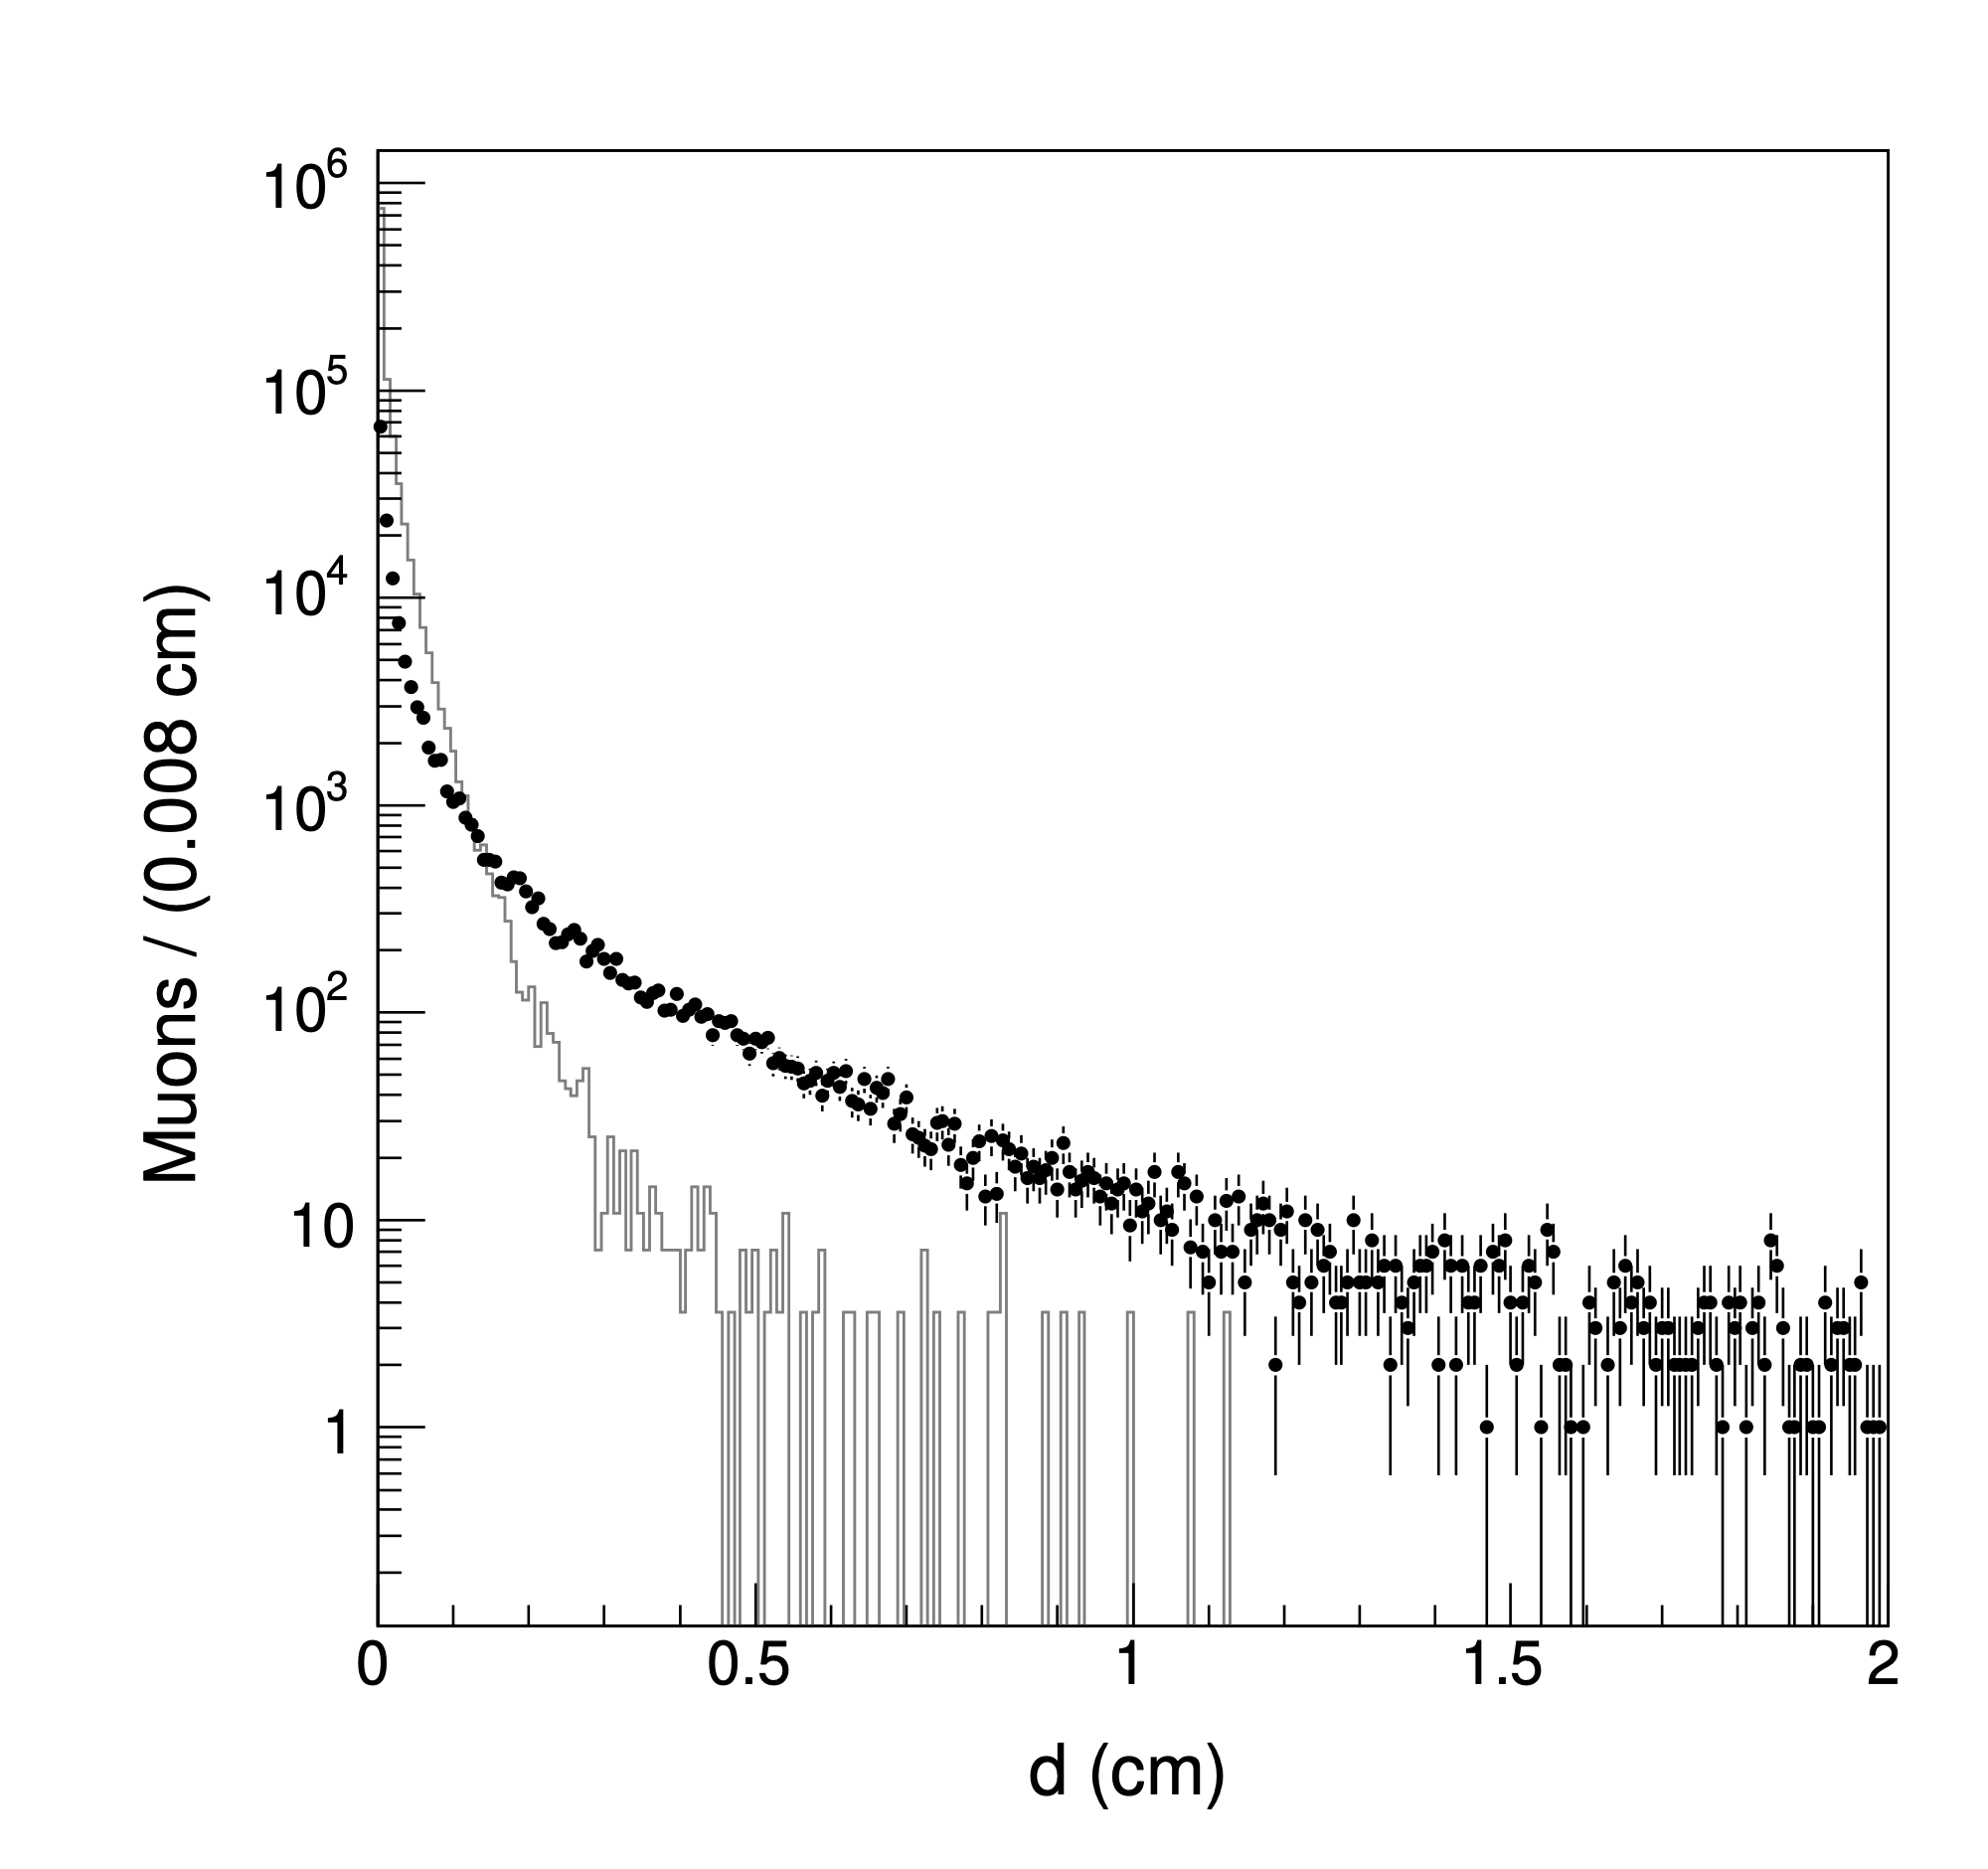
\includegraphics[width=\textwidth]{./figures/MultiMuons1BW_CDF.png}
        %\caption[] {Impact parameter distribution of muons contributed by ghost
        %  ($\bullet$) and QCD (histogram) events. Muon tracks are
        %  selected with loose SVX requirements. The detector resolution
        %  is $\simeq 30 \; \mu$m, whereas bins are 80 $\mu$m wide.} 
      \end{center}
    \end{figure}
    % ========================
    \end{comment}
  \end{multicols}
\end{multimuons-1}
